\documentclass[a4paper]{bmstu}

\include{preamble}

\bibliography{biblio}

% Переопределяем заголовок титульной страницы, чтобы заменить "бюджетное" на "втаномное"
\renewcommand{\titlepageheader}[2]{
	\begin{wrapfigure}[7]{l}{0.14\linewidth}
		\vspace{3.4mm}
		\hspace{-8mm}
		
\includegraphics[width=0.89\linewidth]{bmstu-logo}
	\end{wrapfigure}
	
	{
		\singlespacing \small
		Министерство науки и высшего образования Российской Федерации \\
		Федеральное государственное автономное образовательное учреждение \\
		высшего образования \\
		<<Московский государственный технический университет \\
		имени Н.~Э.~Баумана \\
		(национальный исследовательский университет)>> \\
		(МГТУ им. Н.~Э.~Баумана) \\
	}
	
	\vspace{-4.2mm}
	\vhrulefill{0.9mm} \\
	\vspace{-7mm}
	\vhrulefill{0.2mm} \\
	\vspace{2.8mm}
	
	{
		\small
		ФАКУЛЬТЕТ \longunderline{<<#1>>} \\
		\vspace{3.3mm}
		КАФЕДРА \longunderline{<<#2>>} \\
	}
}

\begin{document}

\makecourseworktitle
	{Информатика и системы управления}
	{Программное обеспечение ЭВМ и информационные технологии}
	{Загружаемый модуль ядра, позволяющий скрывать файлы или запрещать их изменение, чтение и удаление}
	{ИУ7-72Б}
	{А.~А.~Новиков}
	{Н.~Ю.~Рязанова}
	{}
	{}

\include{0A-task}
% \include{0B-abstract}

\maketableofcontents

\begin{center}
    \textbf{ВВЕДЕНИЕ}
\end{center}
\addcontentsline{toc}{chapter}{ВВЕДЕНИЕ}

Обеспечение безопасного доступа к файлам в операционной системе Linux является актуальной задачей. При работе с файлами в Linux необходимо обеспечивать конфиденциальность данных и предоставлять защиту от вредоносных действий.

Целью данной курсовой работы является разработка загружаемого модуля ядра для ОС Linux, позволяющего скрывать файлы или запрещать их изменение, чтение и удаление. Необходимо предусмотреть возможность ввода пароля для отображения файлов или разрешения операций над ними. Предоставить пользователю возможность задавать список таких файлов.

Для решения поставленной задачи необходимо:
\begin{itemize}
	\item[---] проанализировать возможности перехвата функций ядра Linux;
	\item[---] выбрать системные вызовы, которые необходимо перехватить;
	\item[---] разработать алгоритм перехвата, алгоритмы hook–функций и структуру программного обеспечения;
	\item[---] реализовать программное обеспечение;
	\item[---] исследовать работу ПО.
\end{itemize}

 
\chapter{Аналитический раздел}

\section{Способы перехвата функций ядра}

\subsection{ftrace}

ftrace предоставляет возможности для трассировки функций. С его помощью можно отслеживать контекстные переключения, измерять время обработки прерываний, высчитывать время на активизацию заданий с высоким приоритетом и многое другое~\cite{stevens}.

Ftrace был разработан Стивеном Росгедтом и добавлен в ядро в 2008 году, начиная с версии 2.6.27. Ftrace — фреймворк, предоставляющий отладочный кольцевой буфер для записи данных. Собирают эти данные встроенные в ядро программы–трассировщики~\cite{stevens}.

Работает ftrace на базе файловой системы debugfs, которая в большинстве современных дистрибутивов Linux смонтирована по умолчанию.

Каждую перехватываемую функцию можно описать следующей структурой:

\begin{lstlisting}[language=C, frame=single, numbers=left, caption={Структура ftrace\_book}]
struct ftrace_book {
	const char *name;
	void *function;
	void *original;
	
	unsigned long address;
	struct ftrace_ops ops;
};
\end{lstlisting}


Поля структуры:
\begin{itemize}
	\item[---] name — имя перехватываемой функции;
	\item[---] function — адрес функции–сбергки, которая будет вызываться вместо перехваченной функции;
	\item[---] original — указатель на место, куда следует записать адрес перехватываемой функции, заполняется при установке;
	\item[---] address — адрес перехватываемой функции, заполняется при установке;
	\item[---] ops — служебная информация ftrace.
\end{itemize}

\begin{lstlisting}[language=C, frame=single, numbers=left, caption={Пример заполнения структуры ftrace\_book}]
#define HOOK(_name, _function, _original) \
{ \
	.name = (_name), \
	.function = (_function), \
	.original = (_original), \
}

static struct ftrace_book hooked_functions[] = {
	HOOK("sys_clone",  fh_sys_clone,  kreal_sys_clone),
	HOOK("sys_execve",  fh_sys_execve,  kreal_sys_execve),
};
\end{lstlisting}

\subsection{kprobes}

Kprobes — специализированное API, в первую очередь предназначенное для отладки и трассирования ядра. Этот интерфейс позволяет устанавливать пред- и постобработчики для любой инструкции в ядре, а также обработчики на вход и возврат из функции. Обработчики получают доступ к регистрам и могут их изменять.

K probes реализуются с помощью точек останова (инструкции int3), внедряемых в исполнимый код ядра, что позволяет устанавливать к probes в любом месте любой функции, если оно известно. Аналогично, kretprobes реализуются через подмену адреса возврата на стеке и позволяют перехватить возврат из любой функции.

При использовании k probes для получения аргументов функции или значений локальных переменных надо знать, в каких регистрах или где на стеке они лежат, и самостоятельно их оттуда извлекать. Для решения данной проблемы существует j probes — надстройка над k probes, самостоятельно извлекающая аргументы функции из регистров или стека и вызывающая обработчик, который должен иметь ту же сигнатуру, что и перехватываемые функция. Однако j probes объявлен устаревшим и удален из современных ядер.

\subsection{Linux Security API}

Linux Security API — интерфейс, созданный для перехвата функций ядра. В критических местах кода ядра расположены вызовы security–функций, которые в свою очередь вызывают коллёски, установленные security–модулем. Security–модуль может анализировать контекст операции и принимать решение о ее разрешении или запрете.

Для Linux Security API характерны следующие ограничения:

\begin{itemize}
	\item[---] security–модули не могут быть загружены динамически, они являются частью ядра и требуют его перекомпиляции;
	\item[---] в системе может быть только один security–модуль.
\end{itemize}

Таким образом, для использования Security API необходимо поставлять собственную сборку ядра, а также интегрировать дополнительный модуль с SELinux или AppArmor, которые используются популярными дистрибутивами.

\subsection{Модификация таблицы системных вызовов}

В ядре Linux все обработчики системных вызовов хранятся в таблице sys\_call\_table~\cite{linux-kernel}. Подмена значений в этой таблице приводит к смене поведения всей системы. Таким образом, сохранив старое значение обработчика и подставить в таблицу собственный обработчик, можно перехватить системный вызов.

Однако данный подход обладает следующими недостатками:

\begin{itemize}
	\item[---] Техническая сложность реализации, заключающаяся в необходимости обхода защиты от модификации таблицы, атомарное и безопасное выполнение замены.
	\item[---] Невозможность перехвата некоторых обработчиков. В ядрах до версии 4.16 обработка системных вызовов для архитектуры x86\_64 содержала целый ряд оптимизаций. Некоторые из них требовали того, что обработчик системного вызова являлся специальным переходником, реализованным на ассемблере. Соответственно, подобные обработчики порой сложно, а иногда и вовсе невозможно заменить на собственные, написанные на Си~\cite{habr-hooking}.
\end{itemize}

\subsection{Сплайсинг}

Сплайсинг заключается в замене инструкций в начале функции на безусловный переход, ведущий в обработчик. Оригинальные инструкции переносятся в другое место и исполняются перед переходом обратно в перехваченную функцию. Именно таким образом реализуется jump-оптимизация для kprobes. Используя сплайсинг, можно добиться тех же результатов, но без дополнительных расходов на kprobes и с полным контролем ситуации.

Сложность использования сплайсинга заключается в необходимости синхронизации установки и снятия перехвата, обхода защиты от модификации регионов памяти с кодом, инвалидации коней процессора после замены инструкций, дизассемблирования заменяемых инструкций и проверки на отсутствие переходов внутрь заменяемого кода.

\subsection{Сравнительный анализ способов перехвата}

Результаты сравнения различных способов перехвата функций ядра представлены в таблице 1.1

\begin{table}[h]
	\centering
	\caption{Результаты сравнения}
	\begin{tabular}{|p{3cm}|p{3cm}|p{3cm}|p{3cm}|p{3cm}|}
		\hline
		Способ перехвата & Необходимость перекомпиляции ядра & Возможность перехвата любых обработчиков & Доступ к аргументам функции через переменные & Необходимость обхода защиты от модификации регионов памяти \\
		\hline
		Linux Security API & + & --- & + & --- \\
		\hline
		Модификация таблиц системных вызовов & --- & --- & + & + \\
		\hline
		kprobes & --- & + & --- & --- \\
		\hline
		Сплайсинг & --- & + & + & + \\
		\hline
		ftrace & --- & + & + & --- \\
		\hline
	\end{tabular}
\end{table}

\section{Перехватываемые функции ядра}

\subsection{Функция getdents64}

Для сокрытия файла необходимо перехватить функцию ядра getdents64, так как она возвращает записи каталога.

\begin{lstlisting}[language=C, frame=single, numbers=left, caption={Функция getdents64}]
#include <fcntl.h>

int getdents64(unsigned int fd, struct linux_dirent64 *dirp, unsigned int count);
\end{lstlisting}

Системный вызов getdents64 читает несколько структур linux\_dirent64 из каталога, на который указывает открытый файловый дескриптор fd, в буфер, указанный в dirp. В аргументе count задается размер этого буфера.

Структура linux\_dirent64 определена следующим образом:

\begin{lstlisting}[language=C, frame=single, numbers=left, caption={Структура linux\_dirent64}]
struct linux_dirent64 {
	ino64_t    d_ino;
	off64_t    d_off;
	unsigned short  d_reclen;
	unsigned char   d_type;
	char    d_name[];
};
\end{lstlisting}

В d\_ino указан номер inode. В d\_off задается расстояние от начала каталога до начала следующей linux\_dirent64. В d\_reclen указывается размер данной linux\_dirent64. В d\_name задается имя файла, в d\_type — тип файла.

Таким образом, перехват системного вызова getdents64 позволяет удалить запись из списка записей каталога. Перехват вызова осуществляется при помощи создания указателя на системный вызов getdents64.

\begin{lstlisting}[language=C, frame=single, numbers=left, caption={Указатель на getdents64}]
static asmlinkage long (*real_sys_getdents64)(const struct pt_regs *);
\end{lstlisting}

\subsubsection{Функция unlink}

Удаление записей из каталога производится с помощью функции unlink.

\begin{lstlisting}[language=C, frame=single, numbers=left, caption={Функция unlink}]
#include <unistd.h>

int unlink(const char *pathname);
\end{lstlisting}

Эта функция удаляет запись из файла каталога и уменьшает значение счетчика ссылок на файл pathname. Если на файл указывает несколько ссылок, то его содержимое будет через них по-прежнему доступно.

Таким образом, для того, чтобы запретить удаление файла, необходимо перехватить системный вызов unlink. Перехват вызова осуществляется при помощи создания указателя на системный вызов.

\begin{lstlisting}[language=C, frame=single, numbers=left, caption={Указатель на unlink}]
static asmlinkage long (*real_sys_unlinkat)(struct pt_regs *regs);
\end{lstlisting}

\subsubsection{Функции open, write, read}

Запись в файл осуществляется при помощи системного вызова write, чтение из файла — read.

\begin{lstlisting}[language=C, frame=single, numbers=left, caption={Функция write и read}]
#include <fcntl.h>

ssize_t write(int fd, const void *buf, size_t size);
ssize_t read(int fd, void *buf, size_t count);
\end{lstlisting}

Функции write и read работают не с именем файла, а с файловым дескриптором. Однако для того, чтобы определить, можно ли выполнить операцию с файлом, необходимо знать его имя, так как файлы, для которых необходимо запретить те или иные операции, хранятся в виде списка имен этих файлов. Тогда следует перехватить функцию open, которая позволяет получить имя файла.

Системный вызов open осуществляет открытие файла.

\begin{lstlisting}[language=C, frame=single, numbers=left, caption={Функция open}]
#include <fcntl.h>

int open(int dirfd, const char *pathname, int flags);
int open(int dirfd, const char *pathname, int flags, mode_t mode);
\end{lstlisting}

При перехвате open, если имя файла есть в списке, то необходимо сохранить идентификатор процесса, открывающего файл. Затем при перехвате write и read ориентироваться не на имя файла, а на идентификатор процесса и файловый дескриптор. Так можно будет однозначно определить, необходимо ли запретить чтение из файла или запись в него.

Таким образом, для того, чтобы запретить чтение из файла и запись в него, необходимо перехватить системные вызовы open, write и read. Перехват осуществляется при помощи создания указателей на системные вызовы.

\begin{lstlisting}[language=C, frame=single, numbers=left, caption={Указатели на open, write и read}]
static asmlinkage long (*real_sys_open)(struct pt_regs *regs);
static asmlinkage long (*real_sys_write)(struct pt_regs *regs);
static asmlinkage long (*real_sys_read)(struct pt_regs *regs);
\end{lstlisting}

\section{Вывод}

В результате сравнительного анализа выбран способ перехвата функций ядра — ftrace, так как он позволяет перехватывать любые функции ядра и не требует его перекомпиляции. Для сокрытия файла необходимо перехватить функцию getdents64, для запрета чтения из файла и запись в файл — функции open, read и write, удаления — unlink.



\chapter{Конструкторский раздел}

\section{IDEF0}

На рисунке~\ref{fig:idef0} приведена диаграмма состояний IDEF0 нулевого уровня, а на рисунке~\ref{fig:idef01} --- диаграмма состояний IDEF0 первого уровня.

\begin{figure}[H]
	\centering
	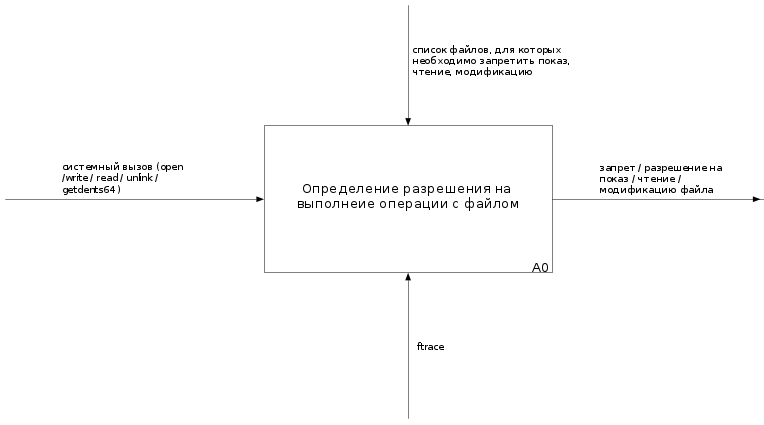
\includegraphics[scale=0.5]{img/01_A0.png}
	\caption{Диаграмма состояний IDEF0 нулевого уровня}
	\label{fig:idef0}
\end{figure}

\begin{figure}[H]
	\centering
	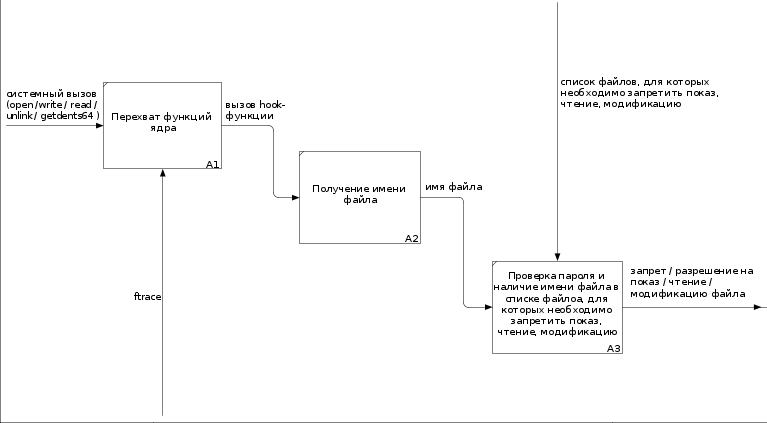
\includegraphics[scale=0.5]{img/02_A0.png}
	\caption{Диаграмма состояний IDEF0 первого уровня}
	\label{fig:idef01}
\end{figure}

\section{Алгоритм проверки необходимости сокрытия файла}

На рисунке~\ref{fig:1} приведена схема алгоритма проверки необходимости сокрытия файла.

\begin{figure}[H]
	\centering
	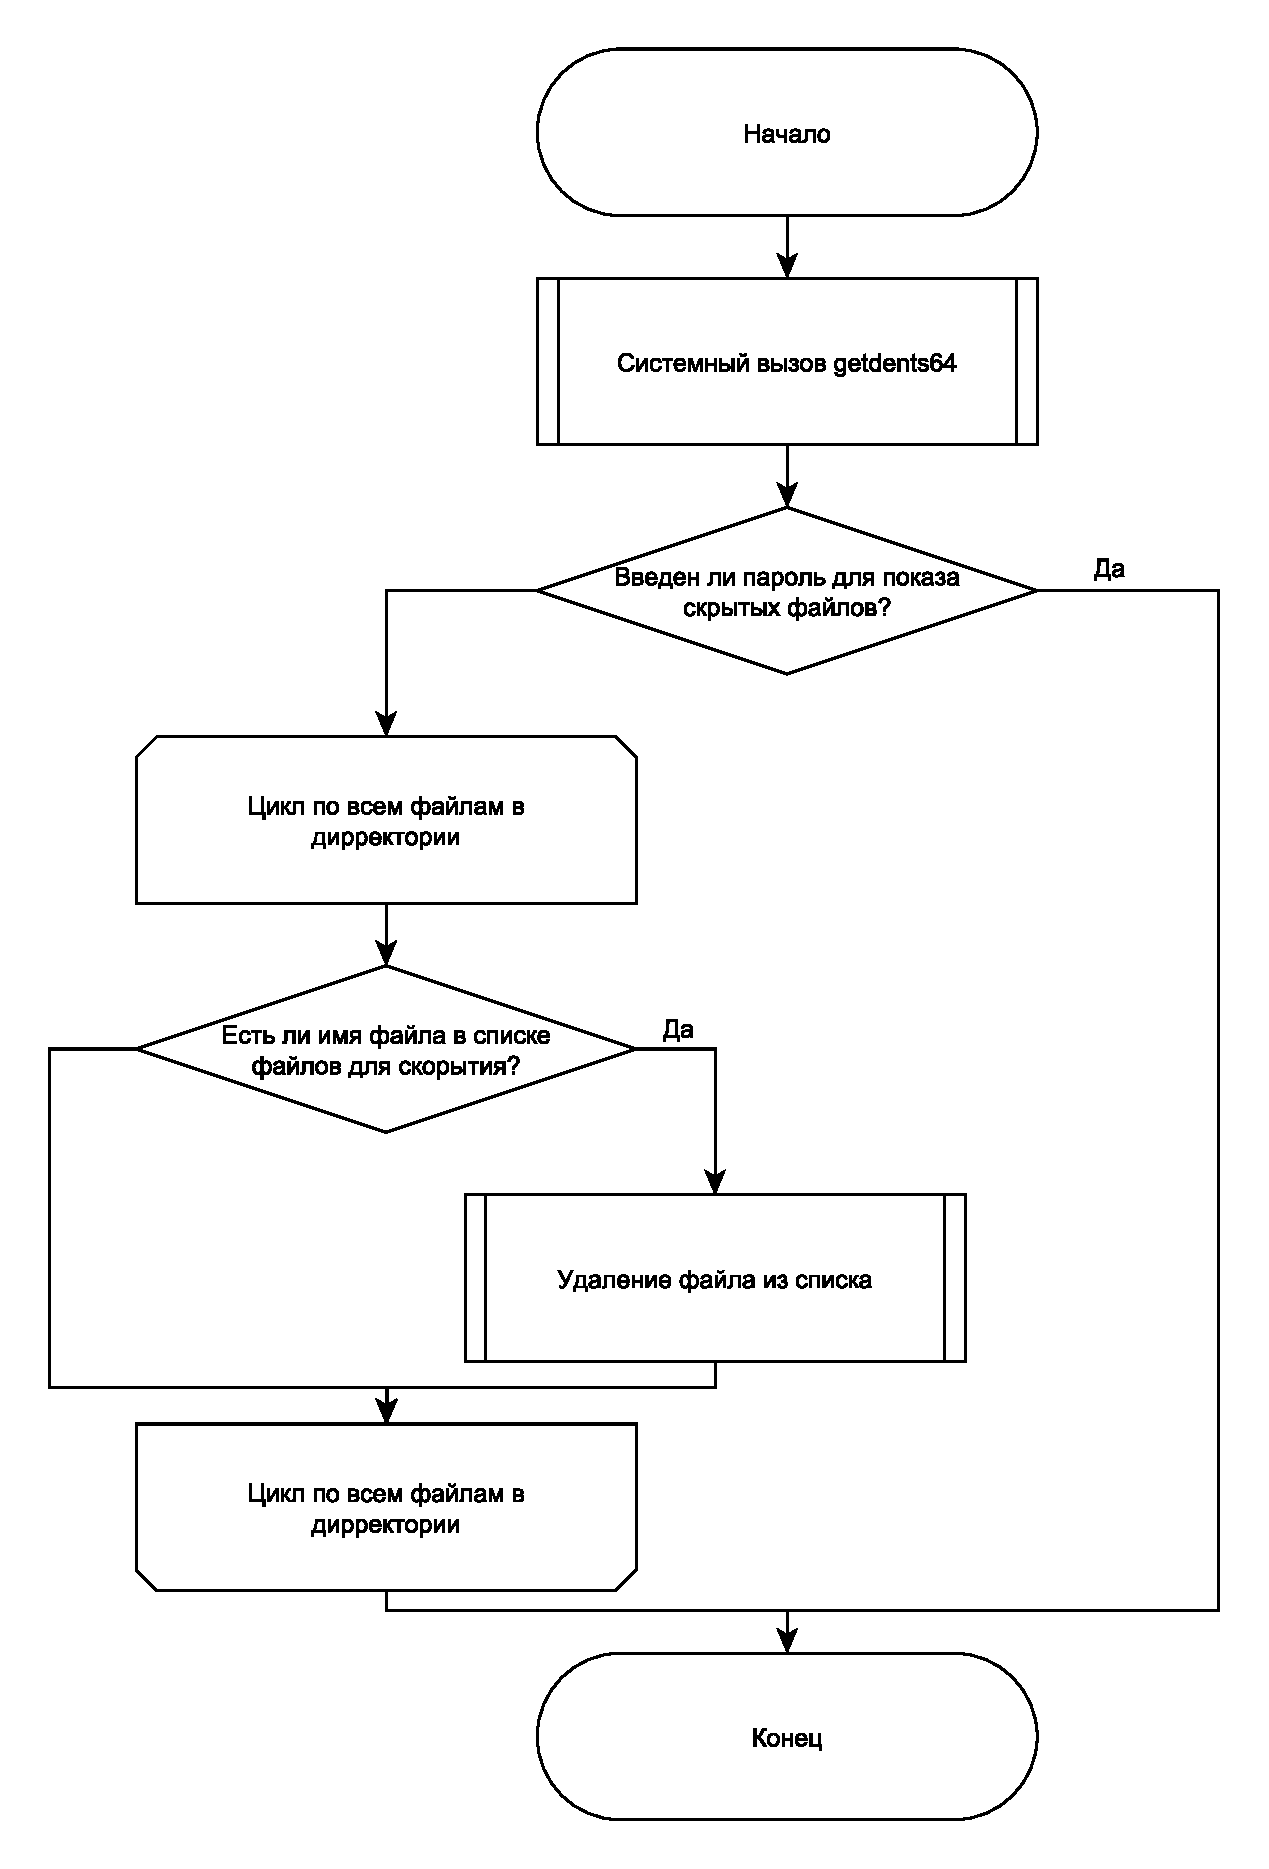
\includegraphics[scale=0.5]{img/first.eps}
	\caption{Алгоритм проверки необходимости сокрытия файла}
	\label{fig:1}
\end{figure}

\section{Алгоритм проверки разрешения на удаление файла}

На рисунке~\ref{fig:2} приведена схема алгоритма проверки разрешения на удаление файла.

\begin{figure}[H]
	\centering
	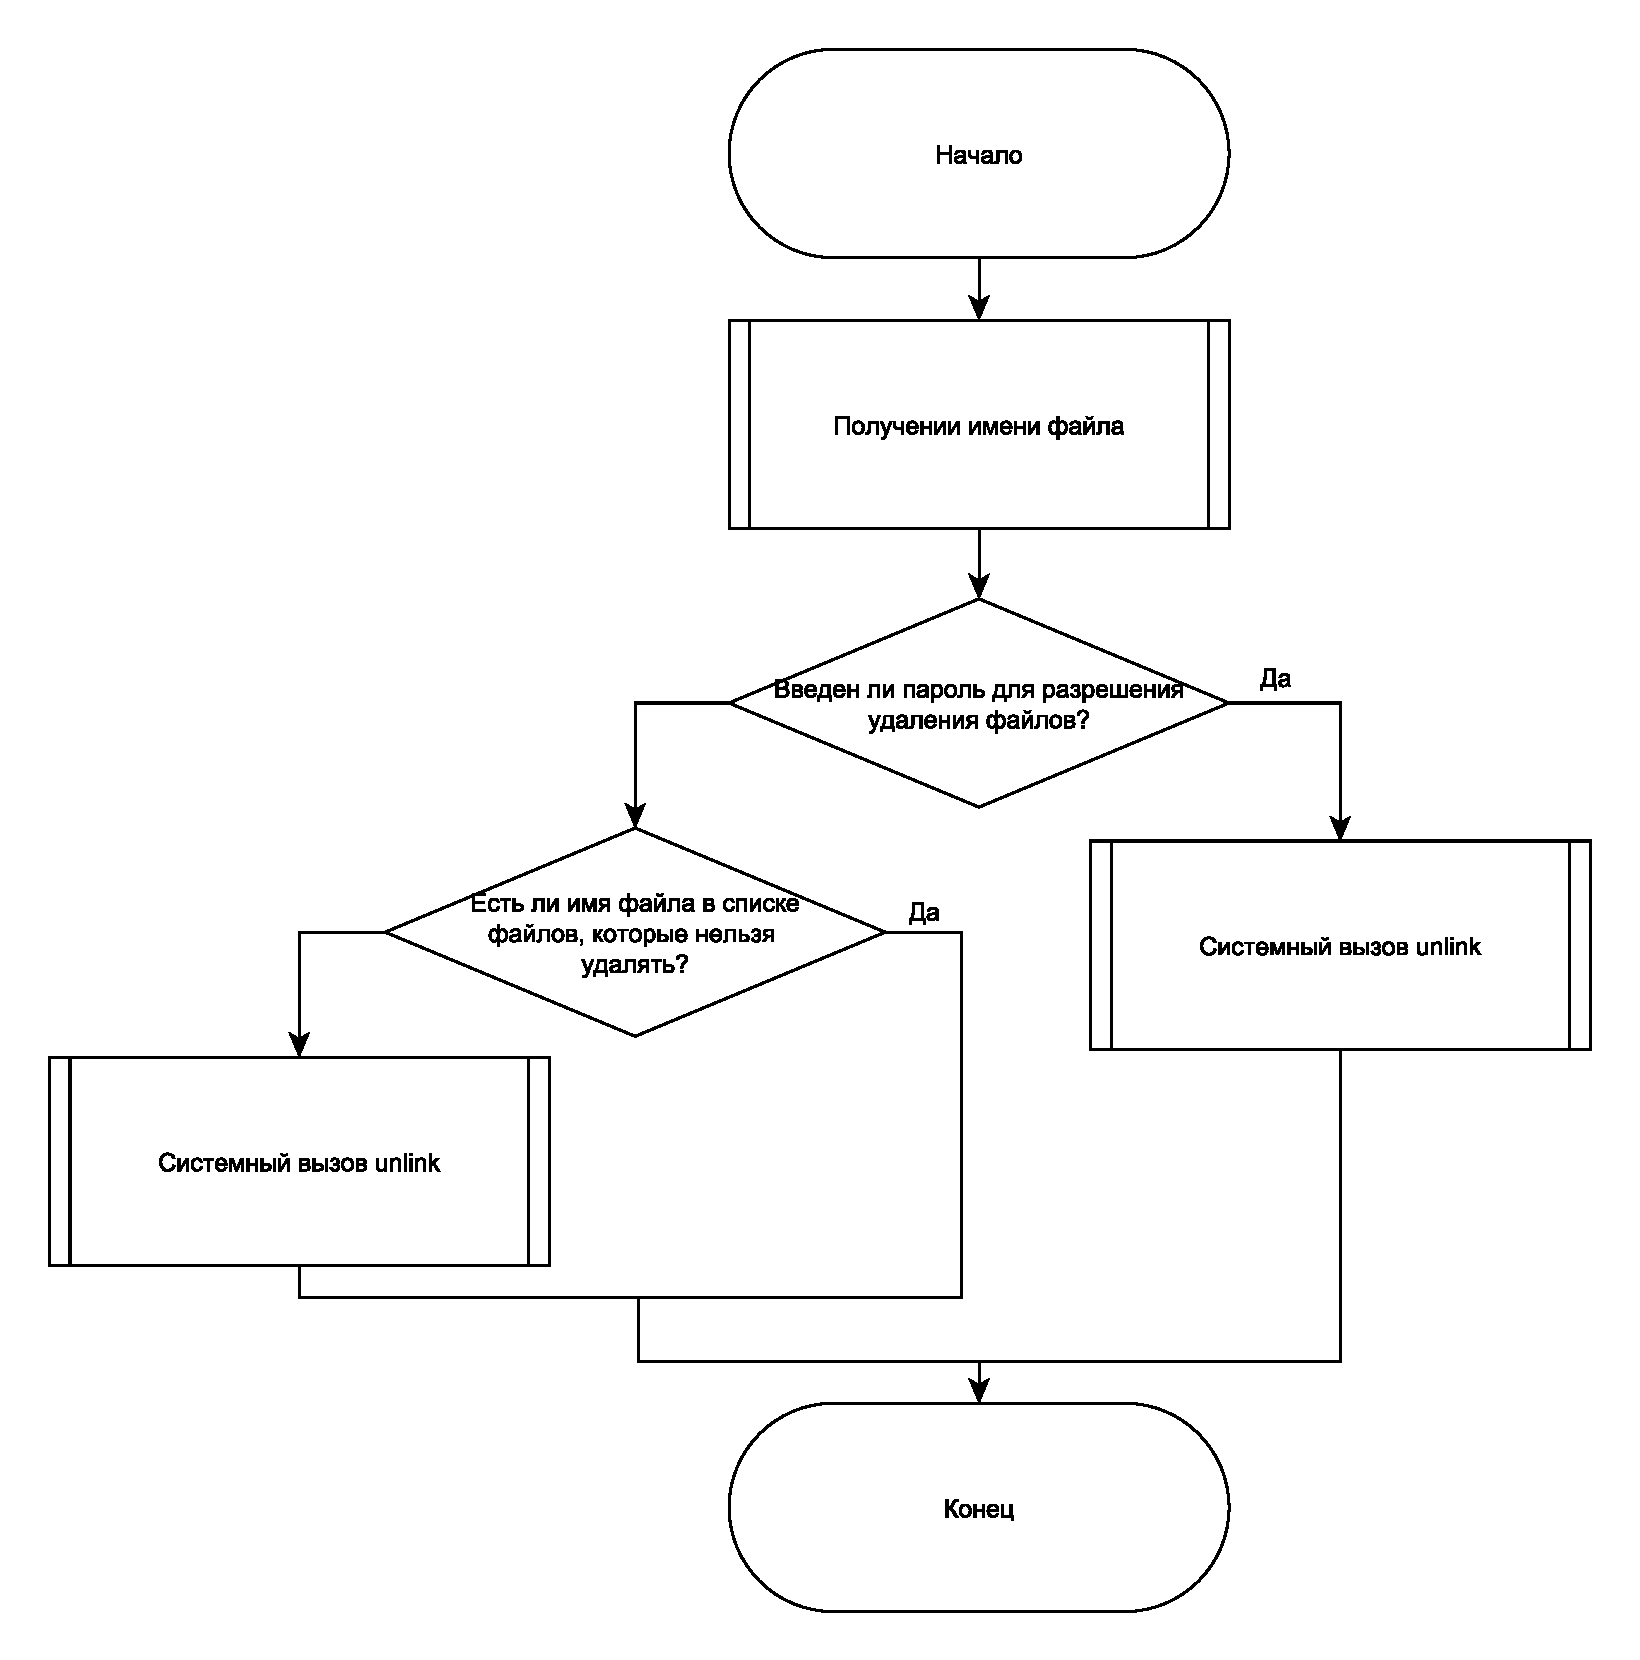
\includegraphics[scale=0.5]{img/second.eps}
	\caption{Алгоритм проверки разрешения на удаление файла}
	\label{fig:2}
\end{figure}

\section{Алгоритм проверки разрешения на запись в файл}

На рисунке~\ref{fig:3} приведена схема алгоритма проверки разрешения на запись в файл.

\begin{figure}[H]
	\centering
	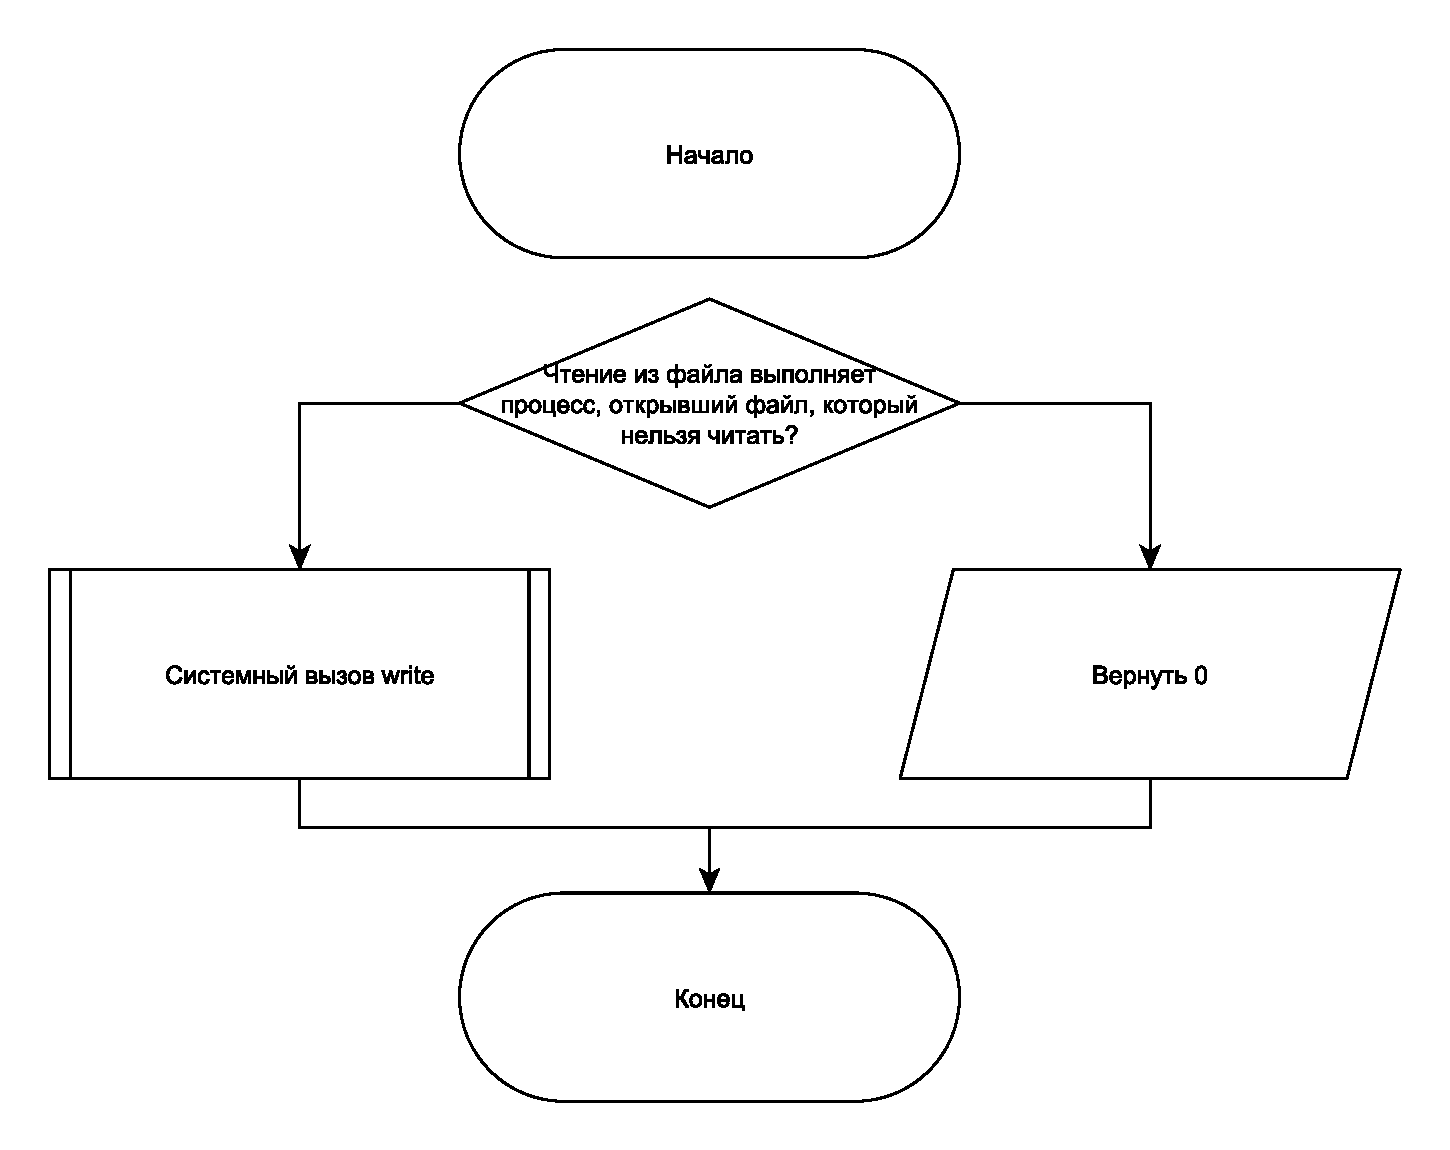
\includegraphics[scale=0.5]{img/third.eps}
	\caption{Алгоритм проверки разрешения на удаление файла}
	\label{fig:3}
\end{figure}

\section{Алгоритм проверки разрешения на чтение из файла}

На рисунке~\ref{fig:4} приведена схема алгоритма проверки разрешения на чтение из файла.

\begin{figure}[H]
	\centering
	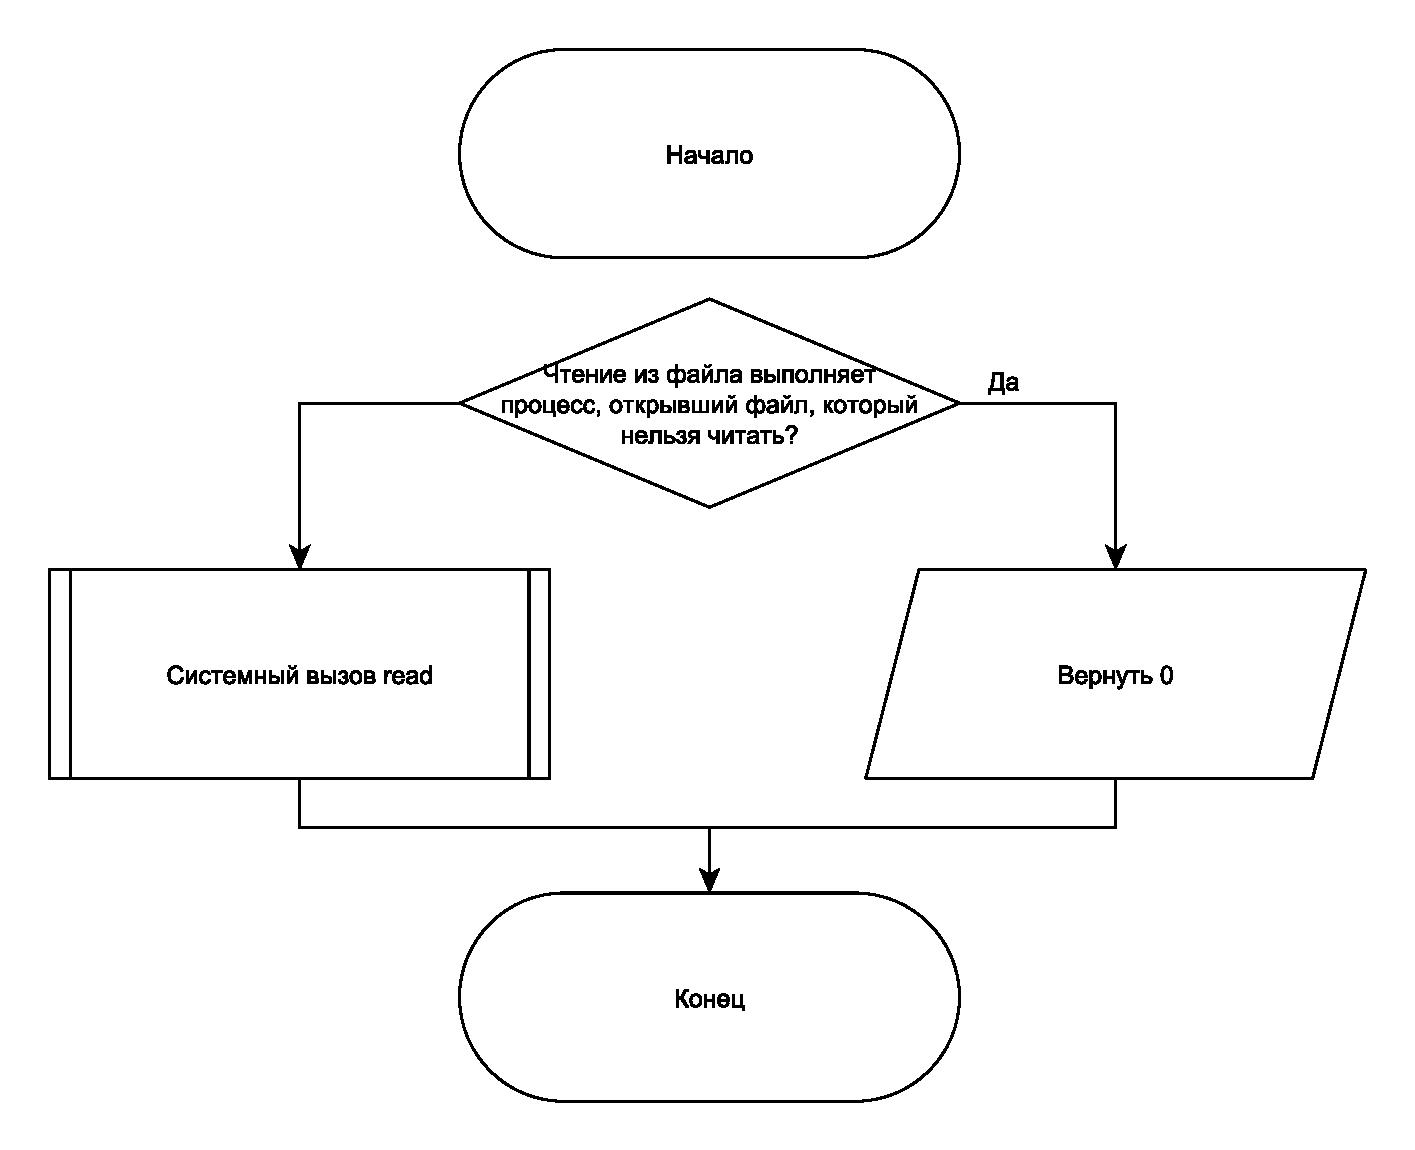
\includegraphics[scale=0.5]{img/fourth.eps}
	\caption{Алгоритм проверки разрешения на удаление файла}
	\label{fig:4}
\end{figure}

\chapter{Технологический раздел}

\section{Выбор языка и среды программирования}

В качестве языка программирования был выбран язык Си. Для сборки модуля использовалась утилита make. В качестве среды программирования был выбран VSCode.

\section{Реализация алгоритма проверки необходимости сокрытия файла}

В листинге 3.1 приведена реализация алгоритма проверки необходимости сокрытия файла.

\begin{lstlisting}[language=C, frame=single, numbers=left, caption={Реализация алгоритма проверки необходимости сокрытия файла}]
static asmlinkage int fh_sys_getdents64(const struct pt_regs *regs)
{
	struct linux_dirent64 __user *dirent = (struct linux_dirent64 *)regs->si;
	struct linux_dirent64 *previous_dir = NULL, *current_dir, *dirent_ker = NULL;
	unsigned long offset = 0;
	int ret = real_sys_getdents64(regs);
	
	if (ret <= 0)
	{
		return ret;
	}
	
	dirent_ker = kmalloc(ret, GFP_KERNEL);
	
	if (dirent_ker == NULL)
	{
		return ret;
	}
	
	if (copy_from_user(dirent_ker, dirent, ret) != 0)
	{
		kfree(dirent_ker);
		return ret;
	}
	
	while (offset < ret)
	{
		current_dir = (struct linux_dirent64 *)((char *)dirent_ker + offset);
		
		if (check_fs_hidelist(current_dir->d_name))
		{
			if (current_dir == dirent_ker)
			{
				ret -= current_dir->d_reclen;
				memmove(current_dir, (void *)current_dir + 
				current_dir->d_reclen, ret);
				continue;
			}
			if (previous_dir)
			{
				previous_dir->d_reclen += current_dir->d_reclen;
			}
		}
		else
		{
			previous_dir = current_dir;
		}
		offset += current_dir->d_reclen;
	}
	if (copy_to_user(dirent, dirent_ker, ret) != 0)
	{
		kfree(dirent_ker);
		return ret;
	}
	kfree(dirent_ker);
	return ret;
}
\end{lstlisting}

\section{Реализация алгоритма проверки разрешения на удаление файла}

Реализация алгоритма проверки разрешения на удаление файла представлена в листинге 3.2.

\begin{lstlisting}[language=C, frame=single, numbers=left, caption={Реализация алгоритма проверки разрешения на удаление файла}]
static asmlinkage long fh_sys_unlink(struct pt_regs *regs)
{
	long ret = 0;
	char *kernel_filename = get_filename((void*) regs->di);
	
	if (!kernel_filename)
	{
		return real_sys_unlink(regs);
	}
	
	if (check_fs_blocklist(kernel_filename))
	{
		ret = 0;
		kfree(kernel_filename);
		return ret;
	}
	
	kfree(kernel_filename);
	ret = real_sys_unlink(regs);
	
	return ret;
}
\end{lstlisting}

\section{Реализация алгоритма проверки разрешения на чтение из файла}

Реализация алгоритма проверки разрешения на чтение из файла представлена в листинге 3.3.

\begin{lstlisting}[language=C, frame=single, numbers=left, caption={Реализация алгоритма проверки разрешения на чтение из файла}]
static asmlinkage long fh_sys_read(struct pt_regs *regs)
{
	long ret = 0;
	struct task_struct *task = current;
	
	if (task->pid == target_pid && regs->di == target_fd)
	{
		return 0;
	}
	
	ret = real_sys_read(regs);
	return ret;
}
\end{lstlisting}

\section{Реализация алгоритма проверки разрешения на запись в файл}

Реализация алгоритма проверки разрешения на запись в файл представлена в листинге 3.4.

\begin{lstlisting}[language=C, frame=single, numbers=left, caption={Реализация алгоритма проверки разрешения на запись в файл}]
static asmlinkage long fh_sys_write(struct pt_regs *regs)
{
	long ret = 0;
	struct task_struct *task;
	task = current;
	
	if (task->pid == target_pid && regs->di == target_fd)
	{
		return 0;
	}
	
	ret = real_sys_write(regs);
	return ret;
}
\end{lstlisting}

\section{Инициализация полей структуры ftrace\_hook}

Инициализация полей структуры ftrace\_hook представлена в листинге 3.5.

\begin{lstlisting}[language=C, frame=single, numbers=left, caption={Инициализация полей структуры ftrace\_hook}]
static struct ftrace_hook demo_hooks[] = {
	HOOK("write", fh_sys_write, &real_sys_write),
	HOOK("read", fh_sys_read, &real_sys_read),
	HOOK("open", fh_sys_open, &real_sys_open),
	HOOK("unlink", fh_sys_unlink, &real_sys_unlink),
	HOOK("getdents64", fh_sys_getdents64, &real_sys_getdents64)
};
\end{lstlisting}

\section{Makefile}

В листинге 3.6 представлен Makefile.

\begin{lstlisting}[language=make, frame=single, numbers=left, caption={Makefile}]
CONFIG_MODULE_SIG=0
PWD := $(shell pwd)
KDIR_PATH ?= /lib/modules/$(shell uname -r)/build

obj-m += my_module.o
my_module-objs := main.o rootkit.o

ccflags-y := -Wall -Wno-unused-result -Wno-unused-function -Wno-unused-variable

all:
$(MAKE) -C $(KDIR_PATH) M=$(PWD) modules

clean:
$(MAKE) -C $(KDIR_PATH) M=$(PWD) clean
\end{lstlisting}


Пример работы разработанного программного обеспечения

После загрузки модуля файлы из списков становятся невидимыми и защищёнными.

\begin{lstlisting}[language=bash, frame=single, numbers=left, caption={Добавление файлов в списки}]
artem@artem-pc:~$ echo hidden.txt   > /proc/hidden
artem@artem-pc:~$ echo protected.txt > /proc/protected
\end{lstlisting}

\begin{lstlisting}[language=bash, frame=single, caption={Содержимое директории после загрузки модуля}]
artem@artem-pc:~/OS_CP$ ls
file.txt  protected.txt
\end{lstlisting}

Файл hidden.txt полностью исчез из листинга.

\begin{lstlisting}[language=bash, caption={Отключение режима скрытия}]
artem@artem-pc:~$ echo 1234 > /dev/emblem
\end{lstlisting}

После ввода пароля 1234 файл снова виден:

\begin{lstlisting}[language=bash, caption={Файлы снова видны}]
artem@artem-pc:~/OS_CP$ ls
file.txt  hidden.txt  protected.txt
\end{lstlisting}

Аналогично, попытка удалить или прочитать protected.txt ничего не даёт:

\begin{lstlisting}[language=bash, caption={Защита от удаления и чтения работает}]
artem@artem-pc:~$ rm protected.txt
artem@artem-pc:~$ echo $?
1
artem@artem-pc:~$ cat protected.txt
(nothing appears)
\end{lstlisting}

Отключаем защиту:

\begin{lstlisting}[language=bash, caption={Отключение режима защиты}]
artem@artem-pc:~$ echo 4321 > /dev/emblem
\end{lstlisting}

Теперь операции проходят успешно:

\begin{lstlisting}[language=bash, caption={Файл снова доступен}]
artem@artem-pc:~$ cat protected.txt
This is a protected file
\end{lstlisting}
\include{5-conclusion}


\makebibliography
\begin{appendices}
	\chapter{}
\end{appendices}

\begin{lstlisting}[language=C, frame=single, numbers=left, caption={Файл main.c}]
#include <linux/module.h>
#include <linux/kernel.h>
#include <linux/init.h>
#include <linux/uaccess.h>
#include <linux/fs.h>
#include <linux/device.h>
#include <linux/cdev.h>
#include <linux/proc_fs.h>
#include <linux/string.h>

#include "rootkit.h"

MODULE_DESCRIPTION("fs_module");
MODULE_AUTHOR("Novikov Artem");
MODULE_LICENSE("GPL");

#define PROC_FILE_NAME_HIDDEN "hidden"
#define PROC_FILE_NAME_PROTECTED "protected"

static char buffer[MAX_BUF_SIZE];
char tmp_buffer[MAX_BUF_SIZE];
char hidden_files[100][100];
int hidden_index = 0;
char protected_files[100][100];
int protected_index = 0;

static ssize_t my_proc_write(struct file *file, const char __user *buf, size_t len, loff_t *ppos)
{
	DBG("my_proc_write called");
	
	if (len > MAX_BUF_SIZE - write_index + 1)
	{
		DBG("buffer overflow");
		return -ENOMEM;
	}
	
	if (copy_from_user(&buffer[write_index], buf, len) != 0)
	{
		DBG("copy_from_user fail");
		return -EFAULT;
	}
	
	write_index += len;
	buffer[write_index - 1] = '\0';
	
	if (strcmp(file->f_path.dentry->d_name.name, PROC_FILE_NAME_HIDDEN) == 0)
	{
		snprintf(hidden_files[hidden_index], len, "%s", &buffer[write_index - len]);
		hidden_index++;
		DBG("file written to hidden %s", hidden_files[hidden_index - 1]);
	}
	else if (strcmp(file->f_path.dentry->d_name.name, PROC_FILE_NAME_PROTECTED) == 0)
	{
		snprintf(protected_files[protected_index], len, "%s", &buffer[write_index - len]);
		protected_index++;
		DBG("file written to protected %s", protected_files[protected_index - 1]);
	}
	else
	{
		DBG("Unknown file->f_path.dentry->d_name.name");
	}
	return len;
}

static ssize_t my_proc_read(struct file *file, char __user *buf, size_t len, loff_t *f_pos)
{
	DBG("my_proc_read called");
	
	if (*f_pos > 0 || write_index == 0)
	return 0;
	
	if (read_index >= write_index)
	read_index = 0;
	
	int read_len = snprintf(tmp_buffer, MAX_BUF_SIZE, "%s\n", &buffer[read_index]);
	
	if (copy_to_user(buf, tmp_buffer, read_len) != 0)
	{
		DBG("copy_to_user error.\n");
		return -EFAULT;
	}
	
	read_index += read_len;
	*f_pos += read_len;
	
	return read_len;
}

static const struct proc_ops fops = {
	.proc_read = my_proc_read,
	.proc_write = my_proc_write,
};

static int __init fh_init(void)
{
	struct device *fake_device;
	int error = 0;
	dev_t dev = 0;
	
	proc_file_hidden = proc_create(PROC_FILE_NAME_HIDDEN, S_IRUGO | S_IWUGO, NULL, &fops);
	if (!proc_file_hidden)
	{
		DBG("call proc_create() fail");
		return -ENOMEM;
	}
	
	proc_file_protected = proc_create(PROC_FILE_NAME_PROTECTED, S_IRUGO | S_IWUGO, NULL, &fops);
	if (!proc_file_protected)
	{
		remove_proc_entry(PROC_FILE_NAME_HIDDEN, NULL);
		DBG("call proc_create() fail");
		return -ENOMEM;
	}
	DBG("proc file created");
	
	error = init_kallsyms();
	if (error) {
		remove_proc_entry(PROC_FILE_NAME_HIDDEN, NULL);
		remove_proc_entry(PROC_FILE_NAME_PROTECTED, NULL);
		DBG("Failed to init kallsyms: %d", error);
		return error;
	}
	
	error = start_hook_resources();
	if (error)
	{
		remove_proc_entry(PROC_FILE_NAME_HIDDEN, NULL);
		remove_proc_entry(PROC_FILE_NAME_PROTECTED, NULL);
		DBG("return in hook functions");
		return error;
	}
	
	error = alloc_chrdev_region(&dev, 0, 1, "table");
	if (error < 0)
	{
		remove_proc_entry(PROC_FILE_NAME_HIDDEN, NULL);
		remove_proc_entry(PROC_FILE_NAME_PROTECTED, NULL);
		return error;
	}
	
	major = MAJOR(dev);
	minor = MINOR(dev);
	
	fake_class = class_create("custom_char_class");
	if (IS_ERR(fake_class)) {
		remove_proc_entry(PROC_FILE_NAME_HIDDEN, NULL);
		remove_proc_entry(PROC_FILE_NAME_PROTECTED, NULL);
		unregister_chrdev_region(dev, 1);
		return PTR_ERR(fake_class);
	}
	
	cdev_init(&fake_cdev, &fake_fops);
	fake_cdev.owner = THIS_MODULE;
	cdev_add(&fake_cdev, dev, 1);
	
	fake_device = device_create(fake_class,
	NULL,
	dev,
	NULL,
	"emblem");
	
	if (IS_ERR(fake_device))
	{
		remove_proc_entry(PROC_FILE_NAME_HIDDEN, NULL);
		remove_proc_entry(PROC_FILE_NAME_PROTECTED, NULL);
		class_destroy(fake_class);
		unregister_chrdev_region(dev, 1);
		return -1;
	}
	
	return 0;
}

static void __exit fh_exit(void)
{
	if (proc_file_hidden)
	{
		remove_proc_entry(PROC_FILE_NAME_HIDDEN, NULL);
		DBG("proc file removed (hidden)");
	}
	
	if (proc_file_protected)
	{
		remove_proc_entry(PROC_FILE_NAME_PROTECTED, NULL);
		DBG("proc file removed (protected)");
	}
	
	fh_remove_hooks(demo_hooks, ARRAY_SIZE(demo_hooks));
	unregister_chrdev_region(MKDEV(major, 0), 1);
	device_destroy(fake_class, MKDEV(major, 0));
	cdev_del(&fake_cdev);
	class_destroy(fake_class);
}

module_init(fh_init);
module_exit(fh_exit);
\end{lstlisting}

\begin{lstlisting}[language=C, frame=single, numbers=left, caption={Файл rootkit.h}]
#ifndef ROOTKIT_H
#define ROOTKIT_H

#include <linux/ftrace.h>
#include <linux/kallsyms.h>
#include <linux/syscalls.h>
#include <linux/kernel.h>
#include <linux/version.h>
#include <linux/delay.h>
#include <linux/kthread.h>
#include <asm/ptrace.h>
#include <linux/fcntl.h>
#include <linux/types.h>
#include <linux/dirent.h>
#include <linux/device.h>
#include <linux/cdev.h>
#include <linux/module.h>
#include <linux/init.h>
#include <linux/fs.h>
#include <linux/proc_fs.h>
#include <linux/kprobes.h>
#include <linux/string.h>

#define FILE_NAME (strrchr(__FILE__, '/') ? strrchr(__FILE__, '/') + 1 : __FILE__)

#define DBG(fmt, ...) \
printk(KERN_INFO "DBG: %s(%d): " fmt "\n", FILE_NAME, __LINE__, ##__VA_ARGS__)

#define MAX_BUF_SIZE 1000

static struct proc_dir_entry *proc_file_hidden;
static struct proc_dir_entry *proc_file_protected;

extern char hidden_files[100][100];
extern int hidden_index;
extern char protected_files[100][100];
extern int protected_index;

static int read_index = 0;
static int write_index = 0;
static unsigned int major;
static unsigned int minor;
static struct class *fake_class;
static struct cdev fake_cdev;
static short fs_hidden = 1;
static short fs_protect = 1;

ssize_t fake_write(struct file *file, const char __user *buf, size_t count, loff_t *offset);

static struct file_operations fake_fops = {
	.write = fake_write,
};

int check_fs_blocklist(char *input);
int check_fs_hidelist(char *input);

static unsigned int target_fd = 0;
static unsigned int target_pid = 0;

typedef unsigned long (*kallsyms_lookup_name_t)(const char *name);
extern kallsyms_lookup_name_t kallsyms_lookup_name_ptr;

int init_kallsyms(void);

static unsigned long lookup_name(const char *name)
{
	if (!kallsyms_lookup_name_ptr) {
		DBG("kallsyms_lookup_name_ptr not initialized");
		return 0;
	}
	return kallsyms_lookup_name_ptr(name);
}

struct ftrace_hook {
	const char *name;
	void *function;
	void *original;
	
	unsigned long address;
	struct ftrace_ops ops;
};

#ifndef MCOUNT_INSN_SIZE
#define MCOUNT_INSN_SIZE 5
#endif

static int fh_resolve_hook_address(struct ftrace_hook *hook)
{
	hook->address = lookup_name(hook->name);
	
	if (!hook->address) {
		DBG("unresolved symbol: %s, trying alternatives\n", hook->name);
		// Попробуем альтернативные имена
		char alt_name[128];
		// Попробуем __do_sys_* вместо __x64_sys_*
		if (strncmp(hook->name, "__x64_sys_", 10) == 0) {
			snprintf(alt_name, sizeof(alt_name), "__do_sys_%s", hook->name + 10);
			hook->address = lookup_name(alt_name);
		}
		// Попробуем sys_* без префикса
		if (!hook->address && strncmp(hook->name, "__x64_sys_", 10) == 0) {
			snprintf(alt_name, sizeof(alt_name), "sys_%s", hook->name + 10);
			hook->address = lookup_name(alt_name);
		}
		if (!hook->address) {
			DBG("unresolved symbol: %s (all alternatives failed)\n", hook->name);
			return -ENOENT;
		}
		DBG("resolved via alternative: %s -> %lx\n", hook->name, hook->address);
	}
	*((unsigned long*) hook->original) = hook->address + MCOUNT_INSN_SIZE;
	
	return 0;
}

static void notrace fh_ftrace_thunk(unsigned long ip, unsigned long parent_ip,
struct ftrace_ops *ops, struct ftrace_regs *fregs)
{
	struct pt_regs *regs;
	struct ftrace_hook *hook = container_of(ops, struct ftrace_hook, ops);
	
	regs = ftrace_get_regs(fregs);
	if (!regs)
	return;
	
	regs->ip = (unsigned long)hook->function;
}

int fh_install_hook(struct ftrace_hook *hook);
void fh_remove_hook(struct ftrace_hook *hook);
int fh_install_hooks(struct ftrace_hook *hooks, size_t count);
void fh_remove_hooks(struct ftrace_hook *hooks, size_t count);

static char *get_filename(const char __user *filename)
{
	char *kernel_filename = NULL;
	kernel_filename = kmalloc(4096, GFP_KERNEL);
	if (!kernel_filename)
	return NULL;
	
	if (strncpy_from_user(kernel_filename, filename, 4096) < 0) {
		kfree(kernel_filename);
		return NULL;
	}
	return kernel_filename;
}

static asmlinkage long (*real_sys_write)(struct pt_regs *regs);
static asmlinkage long fh_sys_write(struct pt_regs *regs)
{
	long ret = 0;
	struct task_struct *task;
	task = current;
	
	if (task->pid == target_pid && regs->di == target_fd)
	{
		return 0;
	}
	
	ret = real_sys_write(regs);
	return ret;
}

static asmlinkage long (*real_sys_read)(struct pt_regs *regs);
static asmlinkage long fh_sys_read(struct pt_regs *regs)
{
	long ret = 0;
	struct task_struct *task = current;
	
	if (task->pid == target_pid && regs->di == target_fd)
	{
		return 0;
	}
	
	ret = real_sys_read(regs);
	return ret;
}

static asmlinkage long (*real_sys_open)(struct pt_regs *regs);
static asmlinkage long fh_sys_open(struct pt_regs *regs)
{
	long ret;
	char *kernel_filename;
	struct task_struct *task;
	task = current;
	kernel_filename = get_filename((void*) regs->di);
	
	if (!kernel_filename)
	{
		return real_sys_open(regs);
	}
	
	if (check_fs_blocklist(kernel_filename))
	{
		DBG("our file is opened by process with id: %d", task->pid);
		DBG("opened file : '%s'", kernel_filename);
		kfree(kernel_filename);
		ret = real_sys_open(regs);
		DBG("fd returned is %ld", ret);
		if (ret >= 0)
		{
			target_fd = ret;
			target_pid = task->pid;
		}
		return ret;
	}
	
	kfree(kernel_filename);
	ret = real_sys_open(regs);
	
	return ret;
}

static asmlinkage long (*real_sys_unlink)(struct pt_regs *regs);
static asmlinkage long fh_sys_unlink(struct pt_regs *regs)
{
	long ret = 0;
	char *kernel_filename = get_filename((void*) regs->di);
	
	if (!kernel_filename)
	{
		return real_sys_unlink(regs);
	}
	
	if (check_fs_blocklist(kernel_filename))
	{
		ret = 0;
		kfree(kernel_filename);
		return ret;
	}
	
	kfree(kernel_filename);
	ret = real_sys_unlink(regs);
	
	return ret;
}

static asmlinkage long (*real_sys_getdents64)(const struct pt_regs *);
static asmlinkage int fh_sys_getdents64(const struct pt_regs *regs)
{
	struct linux_dirent64 __user *dirent = (struct linux_dirent64 *)regs->si;
	struct linux_dirent64 *previous_dir = NULL, *current_dir, *dirent_ker = NULL;
	unsigned long offset = 0;
	int ret = real_sys_getdents64(regs);
	
	if (ret <= 0)
	{
		return ret;
	}
	
	dirent_ker = kmalloc(ret, GFP_KERNEL);
	
	if (dirent_ker == NULL)
	{
		return ret;
	}
	
	if (copy_from_user(dirent_ker, dirent, ret) != 0)
	{
		kfree(dirent_ker);
		return ret;
	}
	
	while (offset < ret)
	{
		current_dir = (struct linux_dirent64 *)((char *)dirent_ker + offset);
		
		if (check_fs_hidelist(current_dir->d_name))
		{
			if (current_dir == dirent_ker)
			{
				ret -= current_dir->d_reclen;
				memmove(current_dir, (void *)current_dir + 
				current_dir->d_reclen, ret);
				continue;
			}
			if (previous_dir)
			{
				previous_dir->d_reclen += current_dir->d_reclen;
			}
		}
		else
		{
			previous_dir = current_dir;
		}
		offset += current_dir->d_reclen;
	}
	if (copy_to_user(dirent, dirent_ker, ret) != 0)
	{
		kfree(dirent_ker);
		return ret;
	}
	kfree(dirent_ker);
	return ret;
}

#define SYSCALL_NAME(name) ("__x64_sys_" name)

#define HOOK(_name, _function, _original) \
{ \
	.name = SYSCALL_NAME(_name), \
	.function = (_function), \
	.original = (_original), \
}

static struct ftrace_hook demo_hooks[] = {
	HOOK("write", fh_sys_write, &real_sys_write),
	HOOK("read", fh_sys_read, &real_sys_read),
	HOOK("open", fh_sys_open, &real_sys_open),
	HOOK("unlink", fh_sys_unlink, &real_sys_unlink),
	HOOK("getdents64", fh_sys_getdents64, &real_sys_getdents64)
};

static int start_hook_resources(void)
{
	int err;
	err = fh_install_hooks(demo_hooks, ARRAY_SIZE(demo_hooks));
	if (err)
	{
		return err;
	}
	return 0;
}

#endif
\end{lstlisting}


\begin{lstlisting}[language=C, frame=single, numbers=left, caption={Файл rootkit.c}]
#include "rootkit.h"

kallsyms_lookup_name_t kallsyms_lookup_name_ptr = NULL;

int init_kallsyms(void)
{
struct kprobe kp = {
.symbol_name = "kallsyms_lookup_name"
};
int ret;
unsigned long addr;

ret = register_kprobe(&kp);
if (ret < 0) {
DBG("register_kprobe failed for kallsyms_lookup_name: %d", ret);
return ret;
}

addr = (unsigned long)kp.addr;
unregister_kprobe(&kp);

if (!addr) {
DBG("Failed to resolve kallsyms_lookup_name address");
return -ENOENT;
}

kallsyms_lookup_name_ptr = (kallsyms_lookup_name_t)addr;
DBG("kallsyms_lookup_name resolved at %lx", addr);
DBG("kallsyms_lookup_name_ptr set to %px", (void *)kallsyms_lookup_name_ptr);
return 0;
}

ssize_t fake_write(struct file *flip, const char __user *buf, size_t count, loff_t *offset)
{
char message[128];
memset(message, 0, 127);

if (copy_from_user(message, buf, 127) != 0)
{
return -EFAULT;
}

if (strstr(message, "1234") != NULL)
{
fs_hidden = fs_hidden ? 0 : 1;
}

if (strstr(message, "4321") != NULL)
{
fs_protect = fs_protect ? 0 : 1;
}

return count;
}

int check_fs_blocklist(char *input)
{
int i = 0;

if (fs_protect == 0)
{
return 0;
}

if (strlen(protected_files[0]) <= 2)
{
return 0;
}

while (i != protected_index)
{
if (strstr(input, protected_files[i]) != NULL)
return 1;
i++;
}

return 0;
}

int check_fs_hidelist(char *input)
{
int i = 0;

if (fs_hidden == 0)
{
return 0;
}

if (strlen(hidden_files[0]) <= 2)
{
return 0;
}

while (i != hidden_index)
{
if (strstr(input, hidden_files[i]) != NULL)
return 1;
i++;
}

return 0;
}

int fh_install_hook(struct ftrace_hook *hook)
{
int error;

error = fh_resolve_hook_address(hook);
if (error)
{
return error;
}

hook->ops.func = fh_ftrace_thunk;
hook->ops.flags = FTRACE_OPS_FL_SAVE_REGS |
FTRACE_OPS_FL_IPMODIFY |
FTRACE_OPS_FL_RECURSION;

error = ftrace_set_filter_ip(&hook->ops, hook->address, 0, 0);
if (error)
{
DBG("ftrace_set_filter_ip() failed: %d\n", error);
return error;
}

error = register_ftrace_function(&hook->ops);
if (error)
{
DBG("register_ftrace_function() failed: %d\n", error);
ftrace_set_filter_ip(&hook->ops, hook->address, 1, 0);
return error;
}
return 0;
}

void fh_remove_hook(struct ftrace_hook *hook)
{
int err;

err = unregister_ftrace_function(&hook->ops);
if (err)
{
DBG("unregister_ftrace_function() failed: %d\n", err);
}

err = ftrace_set_filter_ip(&hook->ops, hook->address, 1, 0);
if (err)
{
DBG("ftrace_set_filter_ip() failed: %d\n", err);
}
}

int fh_install_hooks(struct ftrace_hook *hooks, size_t count)
{
int err;
size_t i;

for (i = 0; i < count; i++) {
err = fh_install_hook(&hooks[i]);
if (err)
{
while (i != 0)
{
fh_remove_hook(&hooks[--i]);
}
return err;
}
}
return 0;
}

void fh_remove_hooks(struct ftrace_hook *hooks, size_t count)
{
size_t i;

for (i = 0; i < count; i++)
{
fh_remove_hook(&hooks[i]);
}
}#include "rootkit.h"

kallsyms_lookup_name_t kallsyms_lookup_name_ptr = NULL;

int init_kallsyms(void)
{
	struct kprobe kp = {
		.symbol_name = "kallsyms_lookup_name"
	};
	int ret;
	unsigned long addr;
	
	ret = register_kprobe(&kp);
	if (ret < 0) {
		DBG("register_kprobe failed for kallsyms_lookup_name: %d", ret);
		return ret;
	}
	
	addr = (unsigned long)kp.addr;
	unregister_kprobe(&kp);
	
	if (!addr) {
		DBG("Failed to resolve kallsyms_lookup_name address");
		return -ENOENT;
	}
	
	kallsyms_lookup_name_ptr = (kallsyms_lookup_name_t)addr;
	DBG("kallsyms_lookup_name resolved at %lx", addr);
	DBG("kallsyms_lookup_name_ptr set to %px", (void *)kallsyms_lookup_name_ptr);
	return 0;
}

ssize_t fake_write(struct file *flip, const char __user *buf, size_t count, loff_t *offset)
{
	char message[128];
	memset(message, 0, 127);
	
	if (copy_from_user(message, buf, 127) != 0)
	{
		return -EFAULT;
	}
	
	if (strstr(message, "1234") != NULL)
	{
		fs_hidden = fs_hidden ? 0 : 1;
	}
	
	if (strstr(message, "4321") != NULL)
	{
		fs_protect = fs_protect ? 0 : 1;
	}
	
	return count;
}

int check_fs_blocklist(char *input)
{
	int i = 0;
	
	if (fs_protect == 0)
	{
		return 0;
	}
	
	if (strlen(protected_files[0]) <= 2)
	{
		return 0;
	}
	
	while (i != protected_index)
	{
		if (strstr(input, protected_files[i]) != NULL)
		return 1;
		i++;
	}
	
	return 0;
}

int check_fs_hidelist(char *input)
{
	int i = 0;
	
	if (fs_hidden == 0)
	{
		return 0;
	}
	
	if (strlen(hidden_files[0]) <= 2)
	{
		return 0;
	}
	
	while (i != hidden_index)
	{
		if (strstr(input, hidden_files[i]) != NULL)
		return 1;
		i++;
	}
	
	return 0;
}

int fh_install_hook(struct ftrace_hook *hook)
{
	int error;
	
	error = fh_resolve_hook_address(hook);
	if (error)
	{
		return error;
	}
	
	hook->ops.func = fh_ftrace_thunk;
	hook->ops.flags = FTRACE_OPS_FL_SAVE_REGS |
	FTRACE_OPS_FL_IPMODIFY |
	FTRACE_OPS_FL_RECURSION;
	
	error = ftrace_set_filter_ip(&hook->ops, hook->address, 0, 0);
	if (error)
	{
		DBG("ftrace_set_filter_ip() failed: %d\n", error);
		return error;
	}
	
	error = register_ftrace_function(&hook->ops);
	if (error)
	{
		DBG("register_ftrace_function() failed: %d\n", error);
		ftrace_set_filter_ip(&hook->ops, hook->address, 1, 0);
		return error;
	}
	return 0;
}

void fh_remove_hook(struct ftrace_hook *hook)
{
	int err;
	
	err = unregister_ftrace_function(&hook->ops);
	if (err)
	{
		DBG("unregister_ftrace_function() failed: %d\n", err);
	}
	
	err = ftrace_set_filter_ip(&hook->ops, hook->address, 1, 0);
	if (err)
	{
		DBG("ftrace_set_filter_ip() failed: %d\n", err);
	}
}

int fh_install_hooks(struct ftrace_hook *hooks, size_t count)
{
	int err;
	size_t i;
	
	for (i = 0; i < count; i++) {
		err = fh_install_hook(&hooks[i]);
		if (err)
		{
			while (i != 0)
			{
				fh_remove_hook(&hooks[--i]);
			}
			return err;
		}
	}
	return 0;
}

void fh_remove_hooks(struct ftrace_hook *hooks, size_t count)
{
	size_t i;
	
	for (i = 0; i < count; i++)
	{
		fh_remove_hook(&hooks[i]);
	}
}
\end{lstlisting}



\end{document}